\documentclass{classrep}
\usepackage[utf8]{inputenc}
\usepackage[pdftex]{graphicx}
\usepackage[polish]{babel}
\usepackage{algorithm}
\usepackage{algorithmic}
\usepackage{multicol}
\usepackage{amsmath}
\usepackage{listings}
\usepackage{array}
\usepackage{multirow}
\usepackage{hyperref}
\usepackage{subfigure}

\studycycle{Informatyka, studia dzienne, II st.}
\coursesemester{I}

\coursename{Metody Obliczeniowe Optymalizacji}
\courseyear{2010/2011}

\courseteacher{mgr inż. Łukasz Chomątek}
\coursegroup{czwartek, 14:15}
\svnurl{https://serce.ics.p.lodz.pl/svn/labs/moo/lcjp_cz1415/wacjan/Zadanie5@}

\author{%
  \studentinfo{Michał Janiszewski}{169485} \and
  \studentinfo{Leszek Wach}{169513}
}

\title{Zadanie 5: Metoda zewnętrznej funkcji kary}

\begin{document}

\maketitle

\section{Cel zadania}
Celem zadania było zrealizowanie metody optymalizacji z ograniczeniami. Wariant przydzielony naszej grupie zakładał zrealizowanie tej metody za pomocą zewnętrznej lub wewnętrznej funkcji kary. Zdecydowaliśmy się na metodę zewnętrznej funkcji kary.

\section{Metoda funkcji kary}
Metoda funkcji kary to metoda znajdowania minimów problemów nieliniowych, w przypadku których istnieją pewne ograniczenia dotyczące możliwych rozwiązań. Zakładając, że dany problem nieliniowy dotyczycy zagadnienia produkcji, ograniczenia takie mogą istnieć np. ze względu na dostępną ilość surowców lub maszyn \ppauza interesuje nas odnalezienie takiego minimum, które będzie możliwe do spełnienia wykorzystując posiadane zasoby, bez konieczności nabycia nowych.

Niech dany będzie problem nieliniowy:
\begin{equation}
f(x) : R^n \rightarrow R 
\end{equation}
oraz pewna ilość $m$ ograniczeń $g_i$:
\begin{equation}
 g_i(x) : R^n \rightarrow R_{+}, \hspace{3em} i = 1, 2, \ldots, m
\end{equation}

Każde ograniczenie jest postaci:
\begin{equation}
 g_i(x) = \begin{cases} 0 &\mbox{gdy $x$ jest dopuszczalnym rozwiązaniem} \\
	  g^{'}_i(x) & \mbox{w przeciwnym wypadku}\end{cases}
\end{equation}
gdzie $g^{'}_i(x)$ oznacza koszt przekroczenia ograniczenia $g_i$ i spełnia warunek
\begin{equation}
 g^{'}_i(x) > 0
\end{equation}

Zbiorem rozwiązań dopuszczalnych $X$ nazywać będziemy taki zbiór wartości $x$, dla których każde ograniczenie $g_i$ wynosi 0.

Posiadając powyższe informacje, możemy zmodyfikować początkowy problem $f$ i rozwiązywać zamiast niego problem $P$ zdefiniowany w następujący sposób:
\begin{equation}
 P(x, k) = f(x) + \Phi(x, k)
\end{equation}
gdzie $\Phi$ oznacza funkcję kary.

Wobec funkcji kary stawiane są następujące wymagania:
\begin{enumerate}
 \item $\Phi(x, k^j) = 0, \displaystyle \forall_{x \in X}$
 \item $\Phi(x, k^j) > 0, \displaystyle \forall_{x \notin X}$
 \item $\Phi(x, k^{j + 1}) > \Phi(x, k^j), \displaystyle \forall_{x \notin X}$
 \item $\Phi(x, k^j) \rightarrow \infty \mbox{ przy } k \rightarrow \infty, \displaystyle \forall_{x \notin X}$
\end{enumerate}

W skrócie wymagania te można opisać następująco:
\begin{enumerate}
 \item jeśli $x$ jest dopuszczalne, to nie ponosi żadnej kary,
 \item jeśli $x$ nie jest dopuszczalne, to poniesie dodatnią karę,
 \item kara będzie się zwiększać dla kolejnych kroków wyznaczających to samo $x$,
 \item kara będzie dążyć do nieskończoności w sposób nieograniczony.
\end{enumerate}

Łatwo zauważyć, że metoda ta polega na takiej zmianie poszczególnych wartości funkcji, aby zapewnić, że znalezione minimum znajdowało się w zbiorze $X$.

Punkty 1 i 2 nie wymagają komentarza, w przypadku punktów 3 i 4 załóżmy, że minimalizując $P$, trafiliśmy na minimum leżące poza zbiorem dopuszczalnym. Ponieważ jako warunek stopu wykorzystujemy kryterium stacjonarności, nie zdaży się sytuacja, w której program zwróci pozycję tego minimum.

\section{Implementacja}
Zaimplementowaliśmy zadanie w środowisku obliczeniowym Matlab. Do optymalizacji bez ograniczeń wykorzystaliśmy metodę DFP zrealizowaną w zadaniu 3.

Wykorzystaliśmy metodę kwadratowej zewnętrznej funkcji kary, która opisana jest poniższym wzorem:
\begin{equation}
 \Phi(x, k) = k \displaystyle \sum^{m}_{i = 1} (g_i(x))^2
\end{equation}

Jako parametr $k$ wykorzystaliśmy numer kroku, co jak łatwo zauważyć, spełnia warunek
\begin{equation}
 k^1 < k^2 < k^3 < \ldots < k^j
\end{equation}
który zapewnia spełnienie wymogów 3 i 4 stawianych wobec $\Phi$.

Ograniczenia w naszym podajemy w postaci wektora kolumnowego funkcji, które dla wektora kolumnowego z wartościami $x$ zwracają wartości mniejsze lub równe 0 dla dopuszczalnych $x$, a dla niedopuszczalnych \ppauza dodatnią wartość ograniczenia\footnote{Wartość ta zwiększa się wraz z przekraczaniem ograniczenia.}.

Program rysuje wykres funkcji celu, a także, w miejscach, które przekraczają ograniczenia, zmienia kolor w celu jego uwidocznienia.

\section{Wyniki}
\subsection{Funkcja Schwefela}
Funkcja celu:
\begin{equation}
 - x_1 \cdot \sin(\sqrt{\left|x_1\right|}) - x_2 \cdot \sin(\sqrt{\left|x_2\right|})
\end{equation}

Ograniczenia:
\begin{itemize}
 \item $g_1(x) = -\left(\frac{x_1}{5}\right)^2 - x_2 + 20$
 \item $g_2(x) = \left(\frac{x_1}{5}\right)^2 + x_2 - 60$
\end{itemize}

Punkt startowy: $x = [47; -65]$
Znalezione minimum: $x = [65.5479; -124.8294]$

\subsection{Funkcja testowa 2}
Funkcja celu:
\begin{equation}
 3 + (x_1 - 1.5 \cdot x_2)^2 + (x_2 - 2)^2
\end{equation}

Ograniczenia:
\begin{itemize}
 \item $g_1(x) = -\left(\frac{x_1}{5}\right)^2 - x_2 + 20$
 \item $g_2(x) = \left(\frac{x_1}{5}\right)^2 + x_2 - 60$
\end{itemize}

Punkt startowy: $x = [-15; 30]$
Znalezione minimum: $x = [16.4820; 8.9395]$

\begin{figure}
 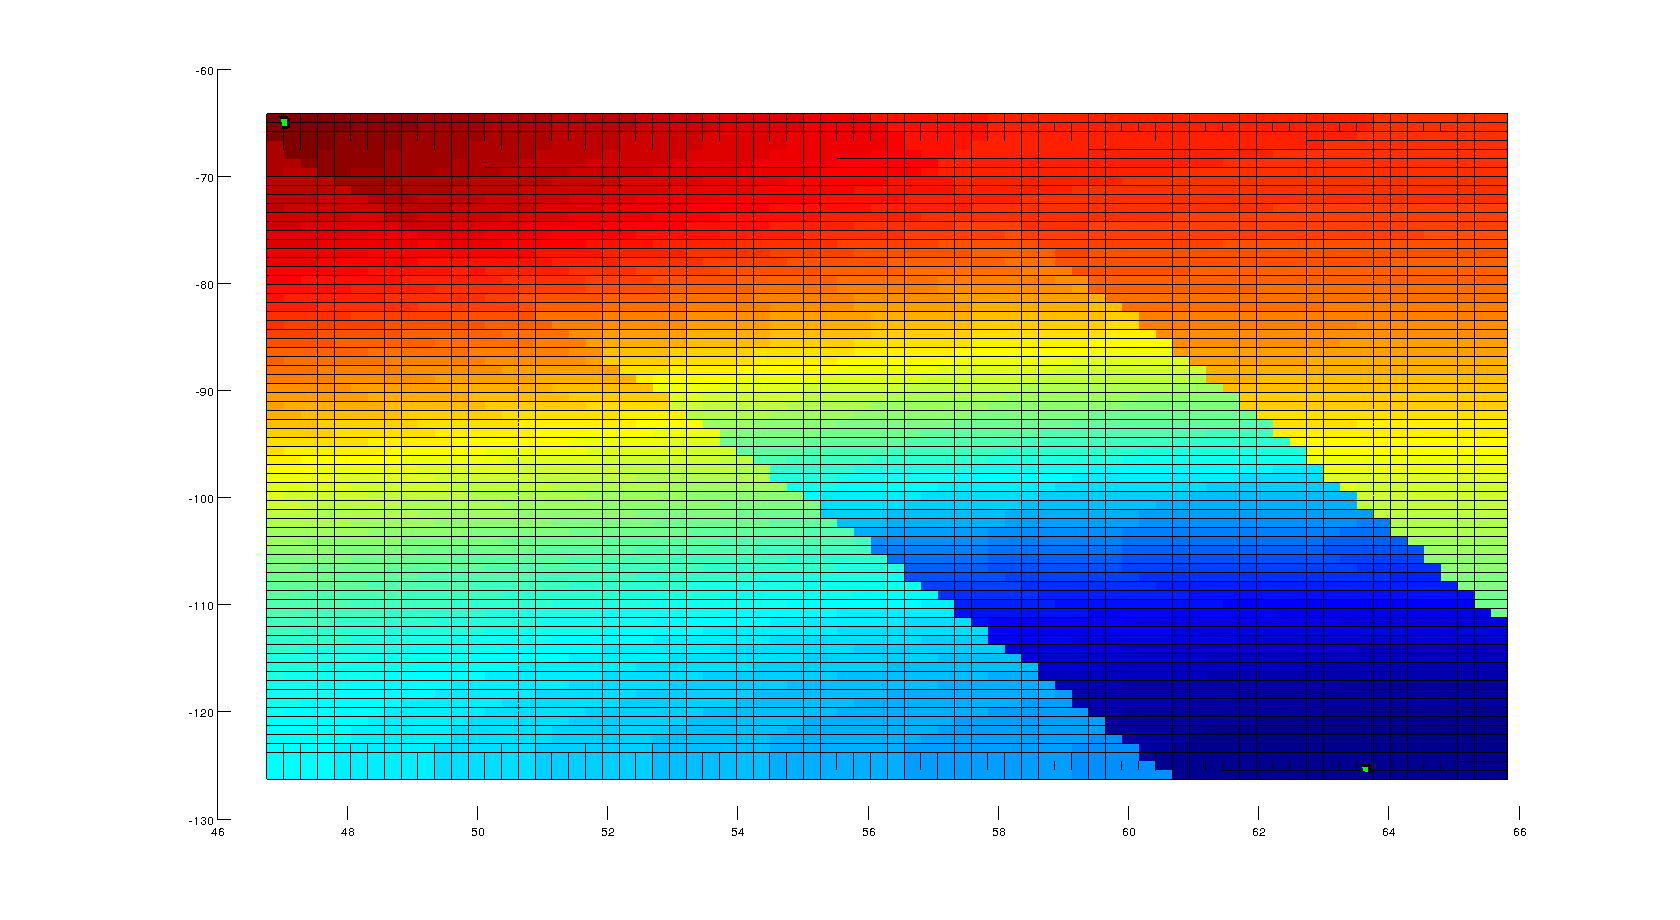
\includegraphics[width=\linewidth]{schwefel}
 \caption{Wynik działania programu dla funkcji Schwefela}
\end{figure}

\begin{figure}
 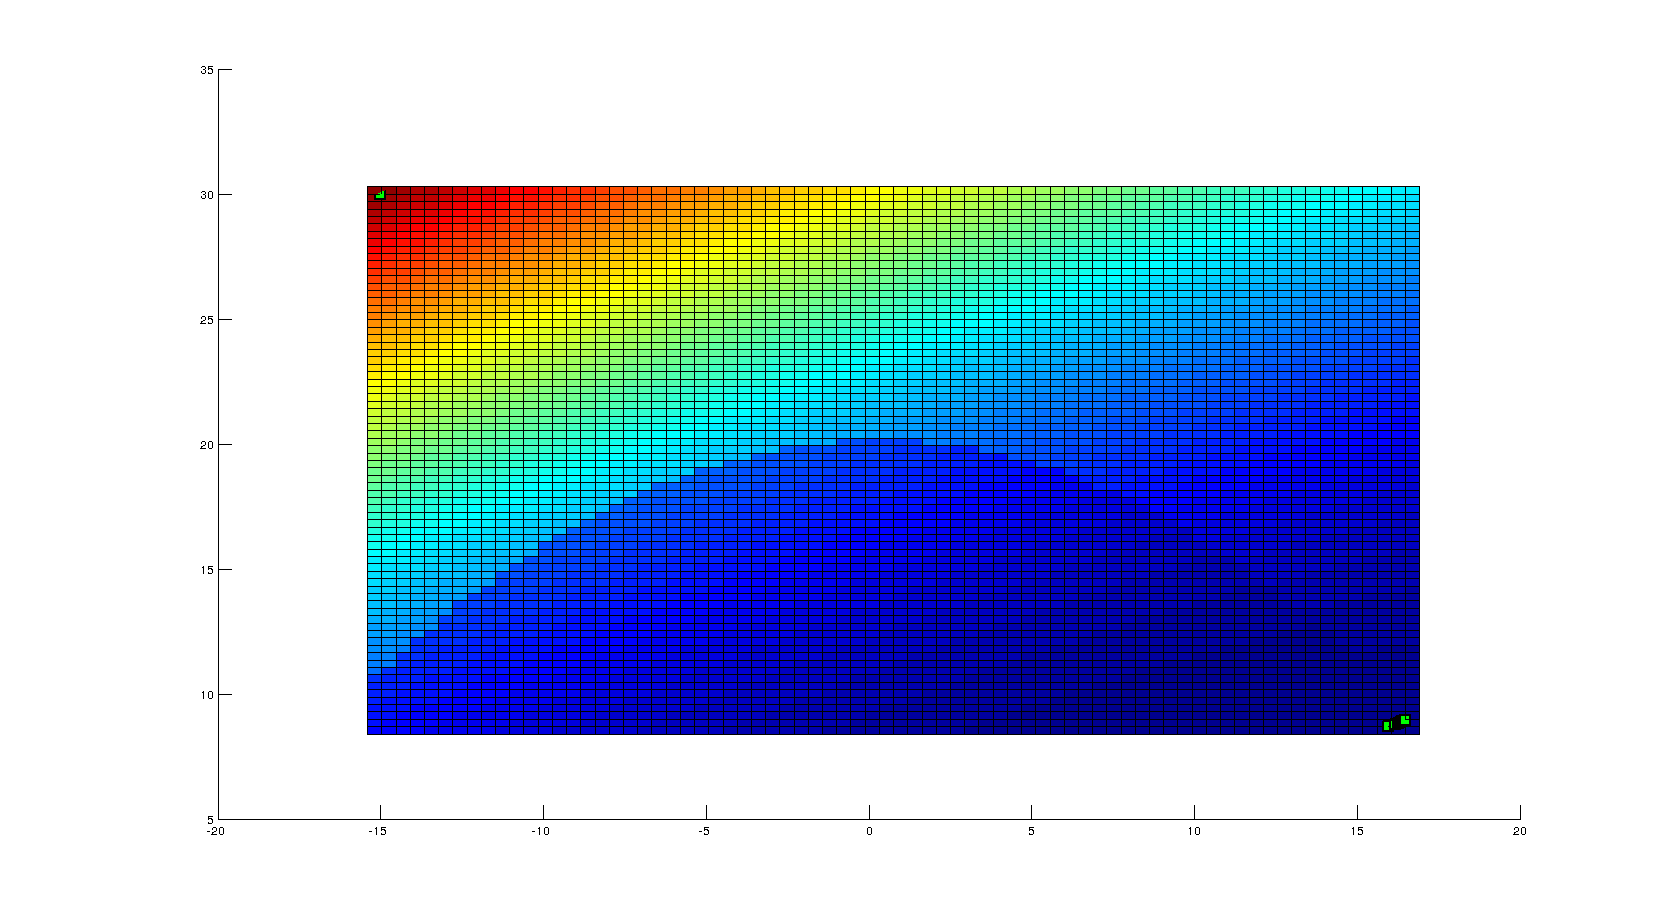
\includegraphics[width=\linewidth]{test2}
 \caption{Wynik działania programu dla funkcji testowej 2}
\end{figure}

\begin{thebibliography}{99}
\bibitem{fkary}
Katedra automatyki, Akademia Górniczo-Hutnicza w Krakowie. \textit{METODA FUNKCJI KARY} [online]. [dostęp 9 czerwca 2011]. Dostępny w internecie: \url{http://aq.ia.agh.edu.pl/Aquarium/labs/opt/fkary.pdf}.
\bibitem{funkcje}
Marcin Molga, Czesław Smutnicki, \textit{Test functions for optimization needs} [online]. [dostęp 9 czerwca 2011]. Dostępny w internecie: \url{http://www.zsd.ict.pwr.wroc.pl/files/docs/functions.pdf}.
\end{thebibliography}

\end{document}
